\documentclass[a4paper]{article}
\usepackage{xunicode}
\usepackage{fontspec}
\usepackage{graphicx}
\usepackage{kpfonts}
\usepackage[T1]{fontenc}


\renewcommand*{\familydefault}{\sfdefault}

\renewcommand{\nobreakspace}{\nobreak\ }

\begin{document}
	\begin{titlepage}
		\begin{center}
		
\includegraphics{logo_fac.png}\\[3.0cm]
		{\Huge ALMA' TWE}\\[0.5cm]
		{\huge\itshape How to loose time with Open ESB}\\[3.0cm]
		\end{center}
		
		\begin{minipage}{0.4\textwidth}
		\begin{flushleft}
			\emph{Authors:}\\[0.1cm]
			Julien \textsc{Durillon}\\
			Alexandre \textsc{Garnier}
		\end{flushleft}
		\end{minipage}
		\begin{minipage}{0.4\textwidth}
		\begin{flushright}
			\emph{Date :}\\[0.1cm]
			\today
		\end{flushright}
		\end{minipage}
		
	\end{titlepage}

	\tableofcontents\clearpage

	\section*{Introduction}
	\addcontentsline{toc}{section}{Introduction}
	
		During this project, we had to specify and develop a distributed application using a Service-Oriented Architecture (SOA).
		The main function of this application is to provide a structure for planning and booking a turn-key week-end in among a set of destinations.
		
		Thus, the principal objectives were here to design and implement services which could permit to build such an architecture on one hand, and to offer a graphical user interface in order to set out the week-end.

	\section{First approach}
	
		\subsection{Main process}
		
		
			The process for using the ALMA TWE service is the following: first, a user looks up for available events matching criteria, such as place or date (figure \ref{fig:lookup}), then book the week-end for the choosen event (figure \ref{fig:mainprocrequest}): travel, hostel, restaurant.
			
			%% Ici figures lookup et mainprocrequest
			\begin{figure}[htp]
				\centering
				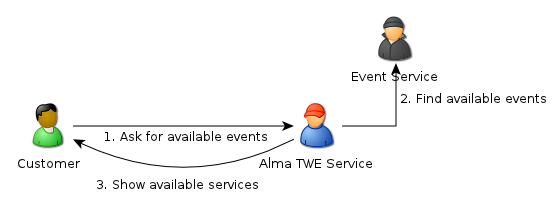
\includegraphics[width=\textwidth]{lookupprocess.png}
				\caption{Event lookup process}
				\label{fig:lookup}
			\end{figure}
			
			\begin{figure}[htp]
				\centering
				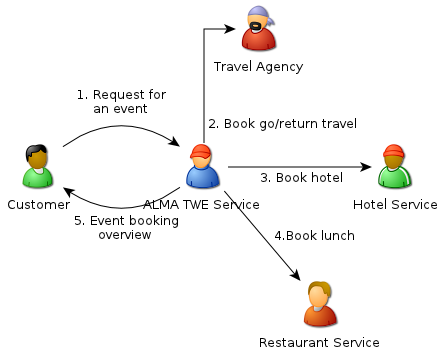
\includegraphics[width=\textwidth]{bookingprocess.png}
				\caption{Event booking process}
				\label{fig:mainprocrequest}
			\end{figure}
			
			
			
		\subsection{Requesting a week-end package}
		
			When the main controller receives a week-end request for an event, it first books the round-up travel, then the hostel for the night, and then the restaurant for the evening lunch before the event. The figure \ref{fig:bookingprocess} describes the whole booking process and the exchanged data.
			
			\begin{figure}[htp]
				\centering
				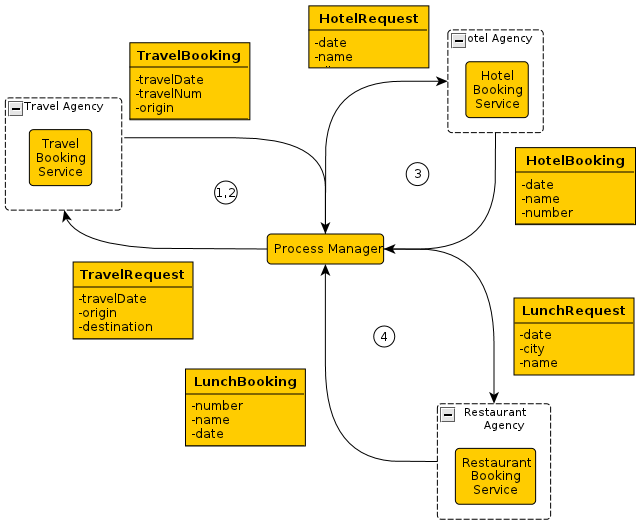
\includegraphics[width=\textwidth]{processmanager.png}
				\caption{Event booking process: with data}
				\label{fig:bookingprocess}
			\end{figure}
			
	
	
	\section{Services}
	
		There are 4 services in the ALMA TWE: Hostel, Restaurant, Event and Travel. All theses services are components of a 5th one : CasaTWE. This one provides a wsdl, that will be used by the user interface.
	
	
	\section{Databases}
	
		\subsection{Database schemes}
		
		The services need databases in order to store and retrieve booking informations. We need then a table for each service that stores available choices, and a table for table for each service that stores booking. The figure \ref{fig:globaldb} describes the differents tables used by the services. Two tables of differents services have no connection between them.
		
		\begin{figure}[htp]
			\centering
			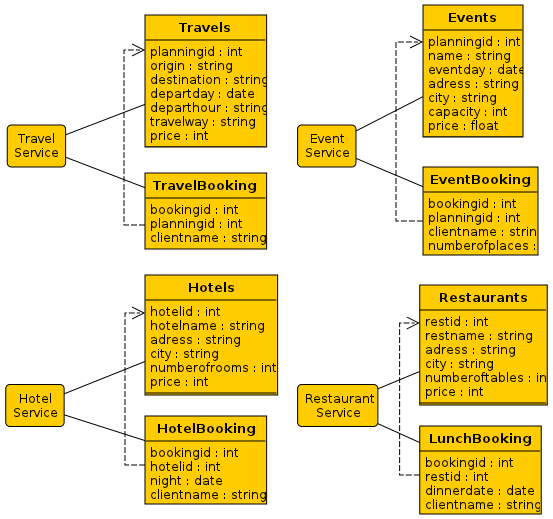
\includegraphics[width=\textwidth]{database.png}
			\caption{Tables for each services}
			\label{fig:globaldb}
		\end{figure}
	
	
	
	\section{User interfaces}
	
		As the implementation presented in this report is still in progress, currently the user interfaces aren't over yet.
		
		Beyond these lack of time issues, we had here to provide a web application that offers to ALMA-TWE clients a graphical user interface to plan and build their turn-key week-ends.
		Moreover, we had to develop a administration interface which permits a total control on databases.
		
		\subsection{Client interface}
		
		As we see in figure \ref{fig:clientiface}, the client interface requires client's data (name, firstname and living town, I presume), the date and destination the client want to travel.
		
		Thus it will then provide him events corresponding to his request. Once he chooses an event, then will be registerred booking to the choosen event, an hotel room, a diner in a restaurant, and the two travels needed to join the destination and then to go home.
		
		Sadly, at this time, some dark technical problems makes this interface cannot communicate with our composite application, despite it recognizes it, and can retrieve and build communication's objects (\emph{ClientRequest} and \emph{ClientBooking}) using the WSDL file using to bind the application with its clients.
		
		\begin{figure}[htp]
			\centering
			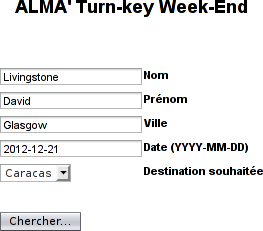
\includegraphics[width=\textwidth/2]{clientiface.png}
			\caption{Tables for each services}
			\label{fig:clientiface}
		\end{figure}
		
		\subsection{Travel map and administration interface}
		
		Moreover, we have still to provide to the client a map that depicts the travel using the OpenStreetMap service.
		
		On the other side, once we get the problems with Client Interface solved, we will develop a similar web application based interface to provides an administrator status who would get full rights on database tables.
	
	\section*{Conclusion}
	\addcontentsline{toc}{section}{Conclusion}

		This project have given to us the opportunity to discover many problematics bound to SOA development, confronting us to choices about services' hierarchy, communications objects, etc.
		
		Beyond that, we spent a very lot of time on using the Open ESB API, which bugs and regular issues forced us many times to reinstall Netbeans, our databases, or even to ``reimplement'' a large part of our ``code'' (if some hundreds of clicks can be considered as an real coding implementation).
		
		Moreover, the development of client and administration interfaces also need a lot of time during the project development, despite their limited interest according to the SOA concepts, and thus to the Services' module.

\end{document}